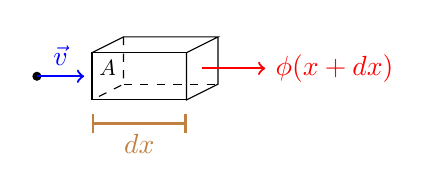
\begin{tikzpicture}




\draw (-0.5,-0.3) node (v6) {} -- (-0.5,0.3) node (v2) {} -- (-0.1,0.5) node (v5) {} -- (1.1,0.5) node (v1) {} -- (0.7,0.3) -- (0.7,-0.3) node (v3) {} -- (1.1,-0.1) node (v8) {} -- (v1.center);
\draw  (v2) rectangle (v3);
\draw [fill] (-1.2,0) node (v4) {} circle (0.05);
\draw [blue, thick,->] (v4.center) -- (-0.6,0)node [midway,above]{$\vec{v}$};
\draw [|-|, thick, brown](-0.5,-0.6) -- (0.7,-0.6)node [midway,below]{$dx$};
\draw [red, thick,->] (0.9,0.1) -- (1.7,0.1)node [right]{$\phi(x+dx)$};
\draw [dashed] (v5.center) -- (-0.1,-0.1) node (v7) {} -- (v6.center);
\draw [dashed](v7.center) -- (v8.center);
\node at (-0.3,0.1) [scale=0.8] {$A$};
\end{tikzpicture}